\documentclass[9pt,a4paper,oneside]{book}

\usepackage[left=2.5cm,right=2.5cm,top=2.5cm,bottom=3cm]{geometry}
\usepackage[utf8]{inputenc}
\usepackage{gentium}
\usepackage[T1]{fontenc}
\usepackage{graphicx}
\graphicspath{{../images/}}
\usepackage{hyperref}
\urlstyle{same}
\usepackage{amsmath}
\usepackage{amsfonts}
\usepackage{amssymb}
\usepackage{circuitikz}


% ************** Fancy Headers ************** 
\usepackage{fancyhdr}

% pagestyle definition: plain
\fancypagestyle{plain}{
	\fancyhf{}
	\fancyhead[L]{}
	\fancyhead[R]{\thepage}
	\renewcommand{\headrulewidth}{0pt}
	\renewcommand{\footrulewidth}{0pt}
}

% pagestyle definition: mmatter
\fancypagestyle{mmatter}{
	\fancyhf{}
	\fancyhead[L]{\leftmark}
	\fancyhead[R]{\thepage}
	\renewcommand{\headrulewidth}{0.5pt}
	\renewcommand{\footrulewidth}{0pt}
}


\begin{document}
\setlength{\parindent}{0pt}
\setlength{\parskip}{6pt}


\frontmatter

% Title page
\begin{titlepage}

\vspace*{3cm}

\begin{center}
	\Huge eistoolbox \par
\end{center}
\begin{center}
	\LARGE for \par
\end{center}
\begin{center}
	\Huge MathWorks\textsuperscript{\textregistered} MATLAB \par
\end{center}

\vspace*{2cm}

\begin{center}
	\Large A toolbox for batch fitting of Electrochemical Impedance Spectroscopy data to equivalent circuit models
\end{center} 

\vspace*{2cm}

\begin{center}
	\Huge User Guide \par
\end{center}
\begin{center}
	\LARGE Juan J. Montero-Rodríguez \par
\end{center}

\vspace*{4cm}

\begin{center}
	\Large Version 0.2-104
\end{center}

\end{titlepage}

\clearpage

\tableofcontents


\mainmatter
\pagestyle{mmatter}

\chapter{Introduction}

\textbf{eistoolbox} is a toolbox for MATLAB\textregistered{} used for batch fitting Electrochemical Impedance Spectroscopy (EIS) data to equivalent circuits models.

In EIS the \textbf{impedance} of a sample is observed and recorded at different frequencies, and the impedance is stored as a Bode diagram, with magnitude and phase (polar format). Results can also be stored as real and imaginary parts (rectangular format) and plotted as a Nyquist diagram.

This impedance is commonly fitted to circuit models, selected depending on the physical characteristics of the measured system. The result is a list of \textbf{circuit elements} such as resistors, capacitors and inductors, and a list of \textbf{parameter values}.

The problem is how to calculate these parameters. This is often achieved using \textbf{nonlinear optimization}, and some of the most famous algorithms for fitting EIS data are based on the Complex Nonlinear Least Squares (CNLS) algorithm such as the Levenberg-Marquardt. However there are many algorithms for this end, and they are difficult to implement as they require advanced mathematics.

The present \textbf{eistoolbox} is a collection of algorithms for nonlinear optimization, and a graphical user interface for batch fitting of multiple EIS curves.

\chapter{Theory}


\section{Impedance Spectroscopy}

Electrochemical Impedance Spectroscopy (EIS) measures the complex impedance of a sample as a function of the frequency. The experimental results are stored in two possible formats: polar coordinates (magnitude and phase) or rectangular coordinates (real and imaginary).

\begin{align} \label{impedance}
	Z(f) = R + jX
\end{align}

where R is the resistance and X is the reactance of the sample.

The real part of the impedance is proportional to the resistivity, and the imaginary part is proportional to the permittivity. Both parameters can be calculated directly from the measurements, considering the exact geometry of the electrodes and measurement setup. For parallel plate electrodes, the following equations apply:

\begin{align}
R = \dfrac{\rho L}{A} \label{resistance} \\
C = \dfrac{\epsilon A}{D} \label{capacitance}
\end{align}

The capacitive reactance is given by

\begin{align}
X_C = \dfrac{1}{2\pi{}fC}	\label{reactivecapacitance}
\end{align}

Substituting \eqref{capacitance} and \eqref{reactivecapacitance} into \eqref{impedance} results in the following equation, which describes the impedance in terms of the resistivity and permittivity of the sample between parallel electrodes:

\begin{align}
Z(f) = \dfrac{\rho L}{A} + \dfrac{1}{2\pi{}f} \dfrac{D}{\epsilon A}
\end{align}

Impedance Spectroscopy is also referred as Dielectric Spectroscopy, because it gives information about the dielectric properties of the measured sample.

%\newpage
%\section{Kramers-Kronig Transforms}
%
%Experimental data can be validated using the Kramers-Kronig Transforms.
%
%
%\section{Fitting algorithms}
%
%\subsection{Levenberg-Marquardt}
%

\chapter{Quick Start Guide}

Steps for batch fitting impedance data curves:

1. Add files using the "Add file..." button (supported .CSV or .DTA)

2. Write the circuit string and fitting parameters (circuit string formatting, see Chapter 3)

3. Click the "Fit" button

4. Save the results using the "Save..." button

\section{Graphical User Interface}

\subsection{Main Window}

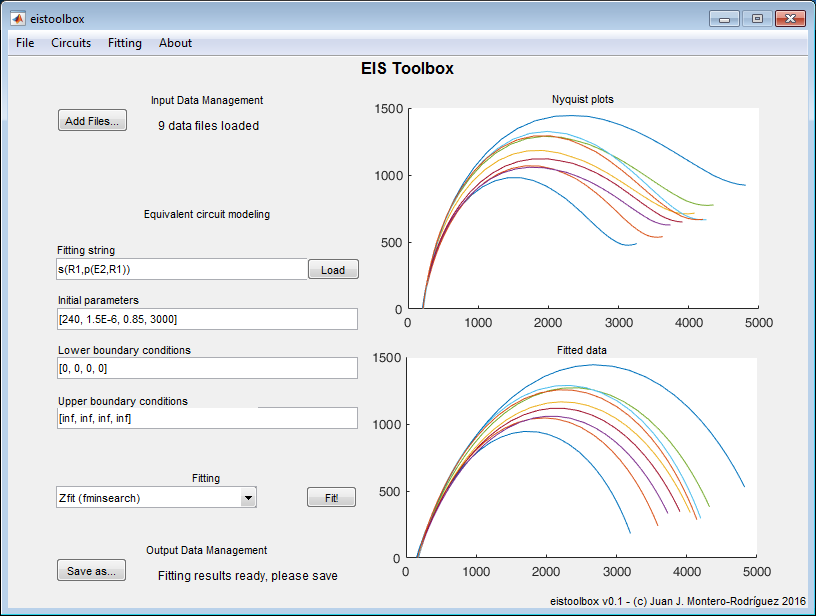
\includegraphics[width=6cm]{main_screenshot.png}

\subsection{Results Window}

The output parameters after the fitting are displayed as a table, in the same order as they appear in the circuit string.

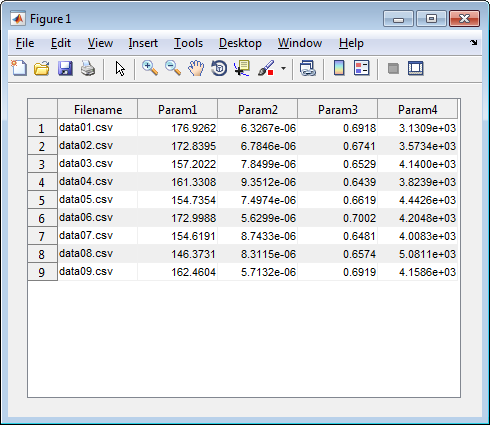
\includegraphics[width=10cm]{scr_results.png}

\subsection{Correlations Window}

This window is useful to validate the fitting results. 

There are three correlations implemented: real, imaginary and magnitude. 

\begin{itemize}
\item The real correlation coefficient (rsq\_real) is obtained by linear regression from the plot of the fitted vs. measured real part of the impedance. 
\item The imaginary correlation coefficient (rsq\_imag) is obtained by linear regression from the plot of the fitted vs. measured imaginary part of the impedance.
\item The magnitude correlation coefficient (rsq\_MAG) is obtained by linear regression from the plot of the fitted vs. measured magnitude of the impedance.	
\end{itemize}

The plots themselves are presented as individual figures. For a perfect fit, the three plots are straight lines where y(x)=x.

Additionally, the fitting results are compared with the original data files by using the Pearson's Chi-square Test of Goodness-of-Fit. This information includes the following parameters: R, chi2, p, fit. These parameters are further explained in Chapter 5.

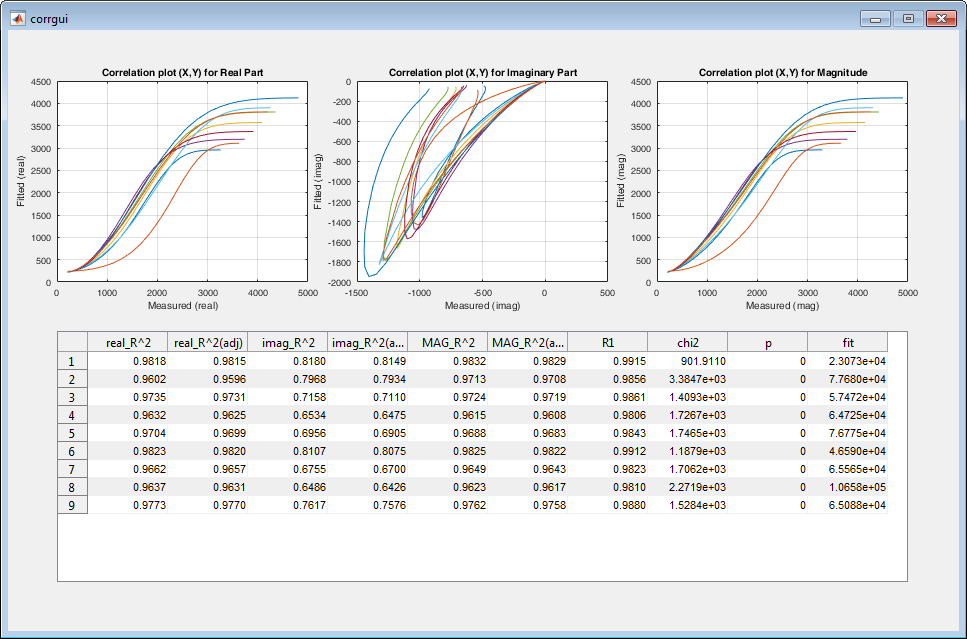
\includegraphics[width=15cm]{correlations.png}






\chapter{Equivalent Circuits}

Experimental data is fitted to equivalent circuit models. The models are designed to describe the interfaces, chemical processes and boundaries of the measured setup.

\subsection{Circuit Elements}

The elements present in the software are described in Table \ref{circelements}:

\begin{table}[h]
	\centering
	\caption{Equivalent circuit elements and their MATLAB implementation.}
	\label{circelements}
	\begin{tabular}{llll}
		\hline \textbf{Symbol} & \textbf{Element} & \textbf{Equation} & \textbf{MATLAB expression}\\
		\hline R1 & Resistor & $Z(f) = R$ & \verb|z=p*ones(size(f))| \\ 
		C1 & Capacitor & $Z(f) = 1 / j 2\pi fC$ & \verb|z=1./(1i*2*pi*f*p)| \\ 
		L1 & Inductor & $Z(f) = j 2\pi fL$  & \verb|z=1i*2*pi*f*p| \\
		E2 & Constant Phase Element & $Z(f) = 1 / p_1 (j 2 \pi f)^{p_2} $ & \verb|z=1./(p(1)*(1i*2*pi*f).^p(2))| \\
		\hline
	\end{tabular}
\end{table}

The Warburg element can be obtained with a Constant-Phase Element by setting $p_2=0.5$


\subsection{Circuit String Syntax}

Circuits can be built using series and parallel combinations of the elements in Table \ref{circelements}, using the series and parallel operators s() and p(). These operators can contain any number of elements, separated by commas.

The number next to the element letter is the number of free parameters for this element. For a capacitor (C1) the only free parameter is the capacitance. For the constant-phase element (E2) the free parameters are p1 and p2.

\textbf{Common mistake:} Do not write the circuit elements as s(R1,R2,R3,C4...). The elements cannot be written as labels. Instead, write s(R1,R1,R1,C1...).

\subsection{Circuit Files (.ckt)}

The circuit string, initial parameters and boundary conditions can be stored and loaded from a circuit file with the .ckt extension. This file is read by MATLAB line-to-line. The file should include only four lines with the following content:

Line 1: circuit string

Line 2: initial parameters, sorted in the same order as they appear in the circuit string

Line 3: lower boundary conditions (LB)

Line 4: upper boundary conditions (UB)

Check the folder 'examples\_circuits' for more examples.

\begin{center}
\fbox{ \parbox{14cm}{
	\textbf{Example 1: Voigt model in the form R+R//C+R//C+R//C}
	
	\begin{circuitikz}
		\draw 
		(0,0) to[R=$R_S$] (2,0)
		(2,0) to[short] (2,2)
		(2,2) to[C=$C_1$] (4,2) % The resistor
		(4,2) to[short] (4,0)
		(2,0) to[R=$R_1$] (4,0)
		(4,0) to[R=$R_2$] (6,0)
		(6,0) to[R=$R_3$] (8,0)
		(4,2) to[C=$C_2$] (6,2)
		(6,2) to[short] (6,0)
		(6,2) to[C=$C_3$](8,2)
		(8,2) to[short] (8,0)
		(8,0) to[short] (10,0);
	\end{circuitikz}
	
	\vspace{5mm}
	\textbf{Recommended circuit file}
	
	s(R1,p(R1,C1),p(R1,C1),p(R1,C1))
	
	[100,100,1e-6,100,1e-6,100,1e-6]
	
	[0,0,0,0,0,0,0]
	
	[inf,inf,inf,inf,inf,inf,inf]
	
	\vspace{5mm}
	\textbf{Notes}
	
	The elements appear in the circuit string in the following order: RS,R1,C1,R2,C2,R3,C3
	
	The initial parameters, LB and UB have the exact same order
	}
}
\end{center}

\begin{center}
	\fbox{ \parbox{14cm}{
			\textbf{Example 2: Ladder circuit in the form: ((((R//C)+R)//C)+R)//C+R}
			
			\begin{circuitikz}
				\draw 
				(6,0) to[R=R3] (8,0)
				(8,0) to[short] (8,2)
				(6,0) to[short] (6,2)
				(6,2) to[C=C3] (8,2)
				(4,2) to[R=R2] (6,2)
				(4,2) to[short] (4,4)
				(4,4) to[C=C2] (6,4)
				(6,4) to[short] (8,4)
				(2,4) to[R=R1] (4,4)
				(2,4) to[short] (2,6)
				(2,6) to[C=C1] (4,6)
				(4,6) to[short] (8,6)
				(0,6) to[R=RS] (2,6)
				(8,6) to[short] (8,0)
				(8,6) to[short] (10,6)
				;
			\end{circuitikz}
			
			\vspace{5mm}
			\textbf{Recommended circuit file}
			
			s(p(s(p(s(p(R1,C1),R1),C1),R1),C1),R1)
			
			[100,1e-6,100,1e-6,100,1e-6,100]
			
			[0,0,0,0,0,0,0]
			
			[inf,inf,inf,inf,inf,inf,inf]
			
			
			\vspace{5mm}
			\textbf{Notes}
			
			The elements appear in the circuit string in the following order: R3,C3,R2,C2,R1,C1,RS
			
			The initial parameters, LB and UB have the exact same order
			
		}
	}
\end{center}


\chapter{Algorithms}

This chapter includes the mathematical description of all the algorithms implemented in the program.

\section{Weighting types}

The fitting algorithms of this toolbox reduce the following distance function (Andrzej Lasia 2014).

\begin{align} \label{distancefun}
dist = S = \sum_{i=1}^{n} \left( w'_i [Z'_i - Z'_{i,calc}]^2 + w''_i [Z''_i - Z''_{i,calc}]^2 \right)
\end{align}

The parameters $w'_i$ and $w''_i$ are the weighting values, computed by one of the following methods:

\begin{tabular}{ll}
	Unit weighting 			& $w'_i = w''_i = 1$ \\
	Modulus weighting 		& $w'_i = w''_i = 1/|Z|^2$ \\
	Proportional weighting 	& $w'_i = 1/(Z')^2$ and $w''_i = 1/(Z'')^2$ \\
	Statistical weighting 	& $w'_i = 1/(\sigma'_i)^2$ and $w''_i = 1/(\sigma''_i)^2$ (not implemented yet)\\
\end{tabular}


\newpage
\section{Minimization algorithms}

\subsection{Nelder-Mead (Simplex)}

The toolbox uses the \textbf{fminsearchbnd} algorithm from John D'Errico.

\subsection{Genetic Algorithm}

ga()

\subsection{Simulated Annealing}

simannealbnd()

\subsection{Constrained Minimization}

fmincon()

\subsection{Other Algorithms}

Not implemented yet

\begin{itemize}
	\item Levenberg-Marquardt
	\item Nelder-Mead
	\item BFGS
	\item Powell
\end{itemize}

\newpage
\section{Statistics}

The overall quality of the fitting can be determined by comparing the original measured data file (expected values) to the simulated values using the fit results (observed values).

Currently the software implements two methods for this comparison: linear regression and Pearson's chi-square test of goodness-of-fit.

\subsection{Linear regressions}

Real of fitted vs Real of measured

Imag of fitted vs Imag of measured

MAG of fitted vs MAG of measured

\subsection{Chi-square}

The Chi-square parameter is calculated with the following equation (Andrzej Lasia 2014).

\[ \chi^2 = \sum_{i=1}^{n}{\left( \left[ \dfrac{Z'_i - Z'_{i,calc}}{\sigma'_i} \right]^2 + \left[ \dfrac{Z''_i - Z''_{i,calc}}{\sigma''_i} \right]^2 \right)} \]

This parameter depends on the number of points.

Usually it is divided by the number of degrees of freedom $\nu = 2N - m$

\[ \chi^2_v = \dfrac{chi^2}{\nu} = \dfrac{chi^2}{2N - m} \]

N is the number of frequencies: there are 2N measured impedance points (N real and N imaginary)

m is the number of adjustable parameters in the model


\subsection{Test F}

For comparing two different variances (Lasia 2014)

Not implemented yet.

\[ F = \dfrac{\sigma_1^2}{\sigma_2^2} \]

\subsection{T-test}

For importance of regression parameters (Lasia 2014)

Not implemented yet.

\[ t = p/s_p \]

where $p$ is the value of the parameter and $s_p$ its standard deviation


\section{Error estimates for individual parameters}

ToDo: This is not yet implemented. It depends on the optimizer functions.

\chapter{Error messages}

\begin{tabular}{lll}
	Error code 	& Error & Details \\
	001			& No data loaded	& There is no input data yet. Add some impedance files in the format FREQ,REAL,IMAG. \\
	002			& Invalid circuit	& The given circuit is not valid. Write using p(), s() and R1,C1,E2 (see chapter 4)\\
\end{tabular}


\newpage{}
\chapter{Licenses for included software}

\section{Zfit}

The original file was released in 2005 and it is available here:\\

\url{https://de.mathworks.com/matlabcentral/fileexchange/19460-zfit}

\begin{small}
\begin{verbatim}
Copyright (c) 2005, Jean-Luc Dellis
All rights reserved.

Redistribution and use in source and binary forms, with or without
modification, are permitted provided that the following conditions are
met:

* Redistributions of source code must retain the above copyright
notice, this list of conditions and the following disclaimer.
* Redistributions in binary form must reproduce the above copyright
notice, this list of conditions and the following disclaimer in
the documentation and/or other materials provided with the distribution

THIS SOFTWARE IS PROVIDED BY THE COPYRIGHT HOLDERS AND CONTRIBUTORS "AS IS"
AND ANY EXPRESS OR IMPLIED WARRANTIES, INCLUDING, BUT NOT LIMITED TO, THE
IMPLIED WARRANTIES OF MERCHANTABILITY AND FITNESS FOR A PARTICULAR PURPOSE
ARE DISCLAIMED. IN NO EVENT SHALL THE COPYRIGHT OWNER OR CONTRIBUTORS BE
LIABLE FOR ANY DIRECT, INDIRECT, INCIDENTAL, SPECIAL, EXEMPLARY, OR
CONSEQUENTIAL DAMAGES (INCLUDING, BUT NOT LIMITED TO, PROCUREMENT OF
SUBSTITUTE GOODS OR SERVICES; LOSS OF USE, DATA, OR PROFITS; OR BUSINESS
INTERRUPTION) HOWEVER CAUSED AND ON ANY THEORY OF LIABILITY, WHETHER IN
CONTRACT, STRICT LIABILITY, OR TORT (INCLUDING NEGLIGENCE OR OTHERWISE)
ARISING IN ANY WAY OUT OF THE USE OF THIS SOFTWARE, EVEN IF ADVISED OF THE
POSSIBILITY OF SUCH DAMAGE.
\end{verbatim}
\end{small}


\section{fminsearchbnd}

This function was written by John D'Errico and published on MathWorks MATLAB Central under an open-source license. The original file can be downloaded at \url{https://de.mathworks.com/matlabcentral/fileexchange/8277-fminsearchbnd--fminsearchcon}.

The function is based on fminsearch and includes the possibility of using boundary conditions, such as the lower and upper limits for the individual circuit parameters.


\end{document}
